\chapter{Detector ATLAS}

\section{Overview}
\begin{figure}[htb]
    \centering
    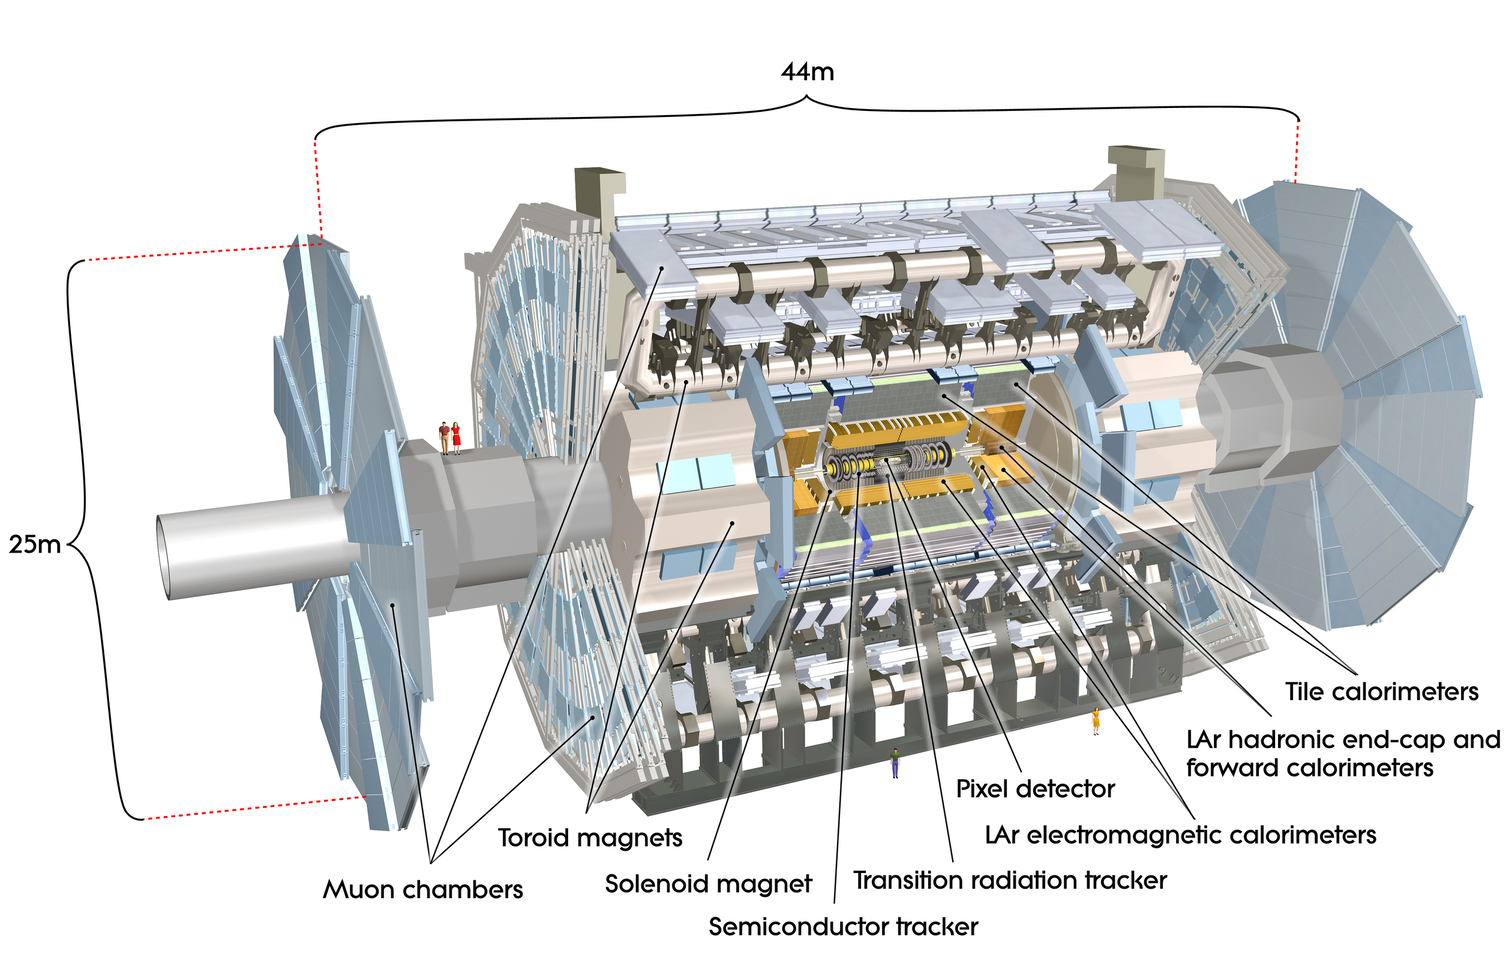
\includegraphics[width=1\linewidth]{src/img/atlas.jpg}
    \caption{The ATLAS detector}
    \label{fig:atlas}
\end{figure}

\LHC is a circular accelerator with a circumference of around 27.6km located on the Swiss-French border near Geneva, at CERN \cite{cern}.
It accelerates particles, mainly protons, occasionally ions (dominantly lead), to almost the speed of light, reaching a center-of-mass energy of $\sqrt{s} = 14$ TeV.
On the accelerating ring are four beam colliding points, where the particles collide and are detected by the ATLAS, \CMS, ALICE, and LHCb detectors.
ATLAS and \CMS are multi-purpose detectors, while ALICE is designed to study heavy-ion collisions, and LHCb is designed to study the physics of b-quarks.


The ATLAS detector \cite{ATLAS} is a general-purpose particle detector located in a cavern 100m underground.
The detector is a multi-layered cylindrical structure with a diameter of 46m and a height of 25m.
The main detecting components are the \emph{silicon pixel and strip trackers}, the \emph{electromagnetic \LAr calorimeter}, the \emph{hadronic calorimeter}, and the \emph{muon spectrometer}.
In \cref{fig:atlas}, we show a schematic of the ATLAS detector, in \cref{fig:tracker,fig:calorimeter,fig:muon,fig:magnet} the individual components, and in \cref{fig:det_inter} the cross section of the detector and its interactions with the particles in individual components.

\begin{figure}[htb]
    \centering
    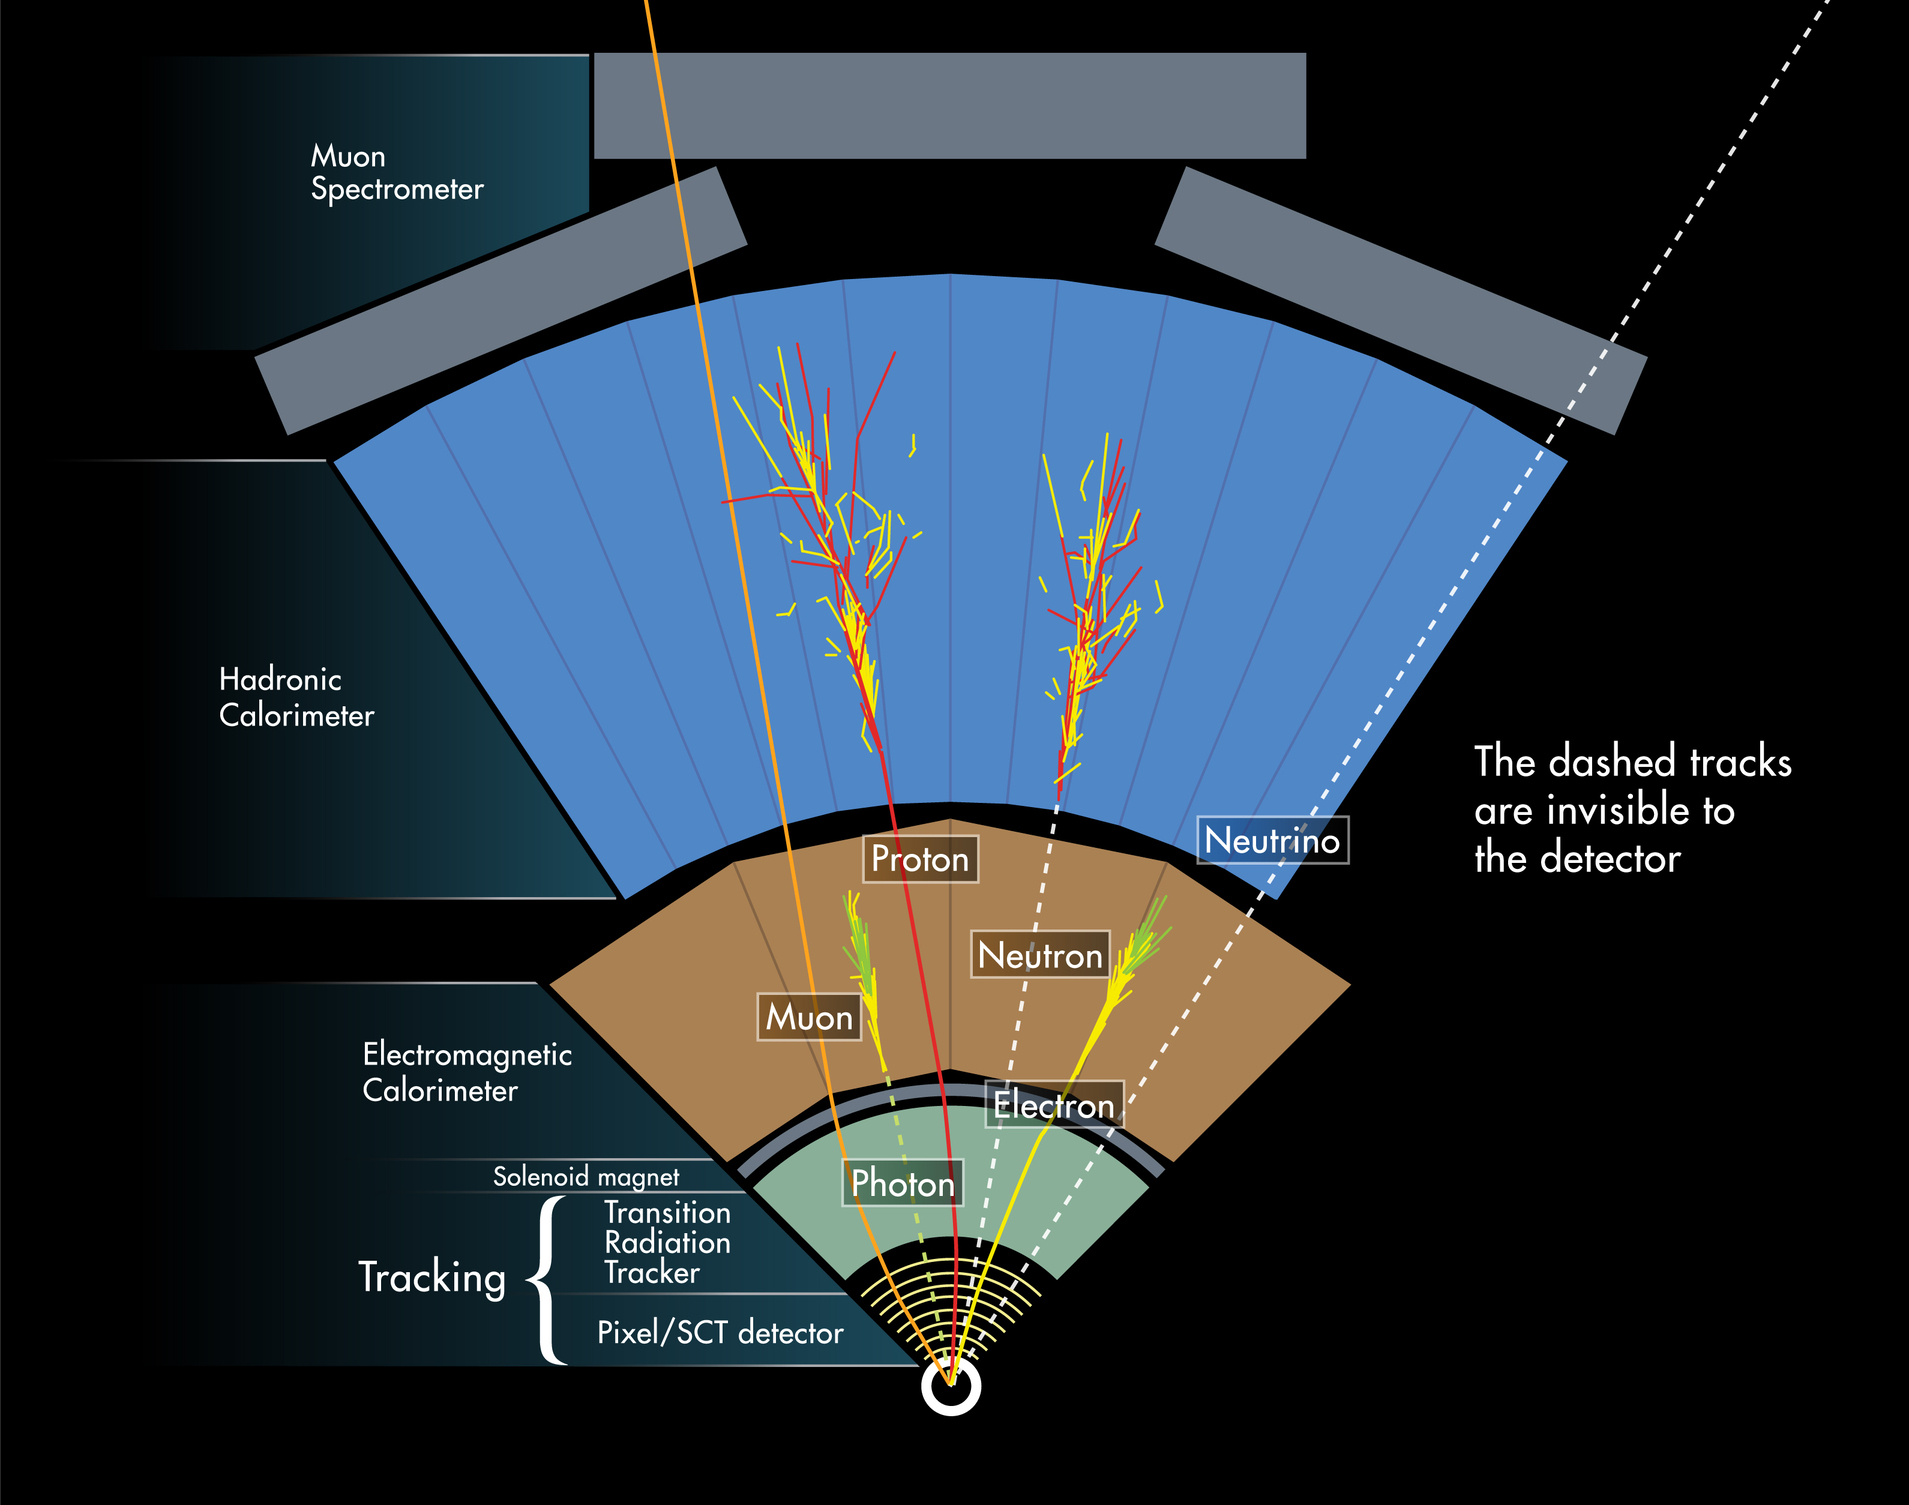
\includegraphics[width=0.9\linewidth]{src/img/det_interactions.jpg}
    \caption{The ATLAS detector cross section and its interactions with the particles.}
    \label{fig:det_inter}
\end{figure}

In the following \cref{sec:lhc}, we will discuss the \LHC and in \cref{sec:trackers,sec:calorimeters,sec:muon,sec:magnet,sec:trigger} the individual components of the detector.
Before doing so, we will introduce the ATLAS coordinate system and space-orienting notation in \cref{sec:atlas_coord}.
\subsection{ATLAS Coordinate System}
\label{sec:atlas_coord}
The ATLAS coordinate system is defined as follows:
\begin{enumerate}
    \item The \emph{origin of the coordinate} system is the nominal interaction point.
    \item The \emph{$z$ axis} is along the beam direction.
    \item the \emph{$x$-$y$ plane} is perpendicular to the beam direction.
    \item The positive \emph{$x$ axis} is pointing towards the centre of \LHC.
    \item The positive \emph{$y$ axis} is pointing upwards.
    \item The \emph{azimuthal angle $\phi$} is measured around the $z$ axis, being zero on the positive $x$ axis.
    \item The \emph{polar angle $\theta$} is measured from the $z$ axis, where is zero.
\end{enumerate}
We also define the \textbf{pseudorapidity} $\eta$ as 
\begin{equation}
    \label{eq:pseudorapidity}
    \eta = -\ln(\tan(\theta/2)),
\end{equation}
and the \textbf{transverse momentum} $\pT$ as momentum in the $x$-$y$ plane.
For massive objects, we also define the \textbf{rapidity} as
\begin{equation}
    \label{eq:rapidity}
    y = \frac{1}{2} \ln\left(\frac{E + p_z}{E - p_z}\right),
\end{equation}
where $E$ is the energy and $p_z$ is the momentum along the $z$ axis of the particle.
The forward region is defined as $|\eta| > 2.5$, and the central region as $|\eta| < 2.5$.

Simple sketches of the ATLAS coordinate system are shown in \cref{fig:atlas_coord}.
\begin{figure}[htb]
    \centering
    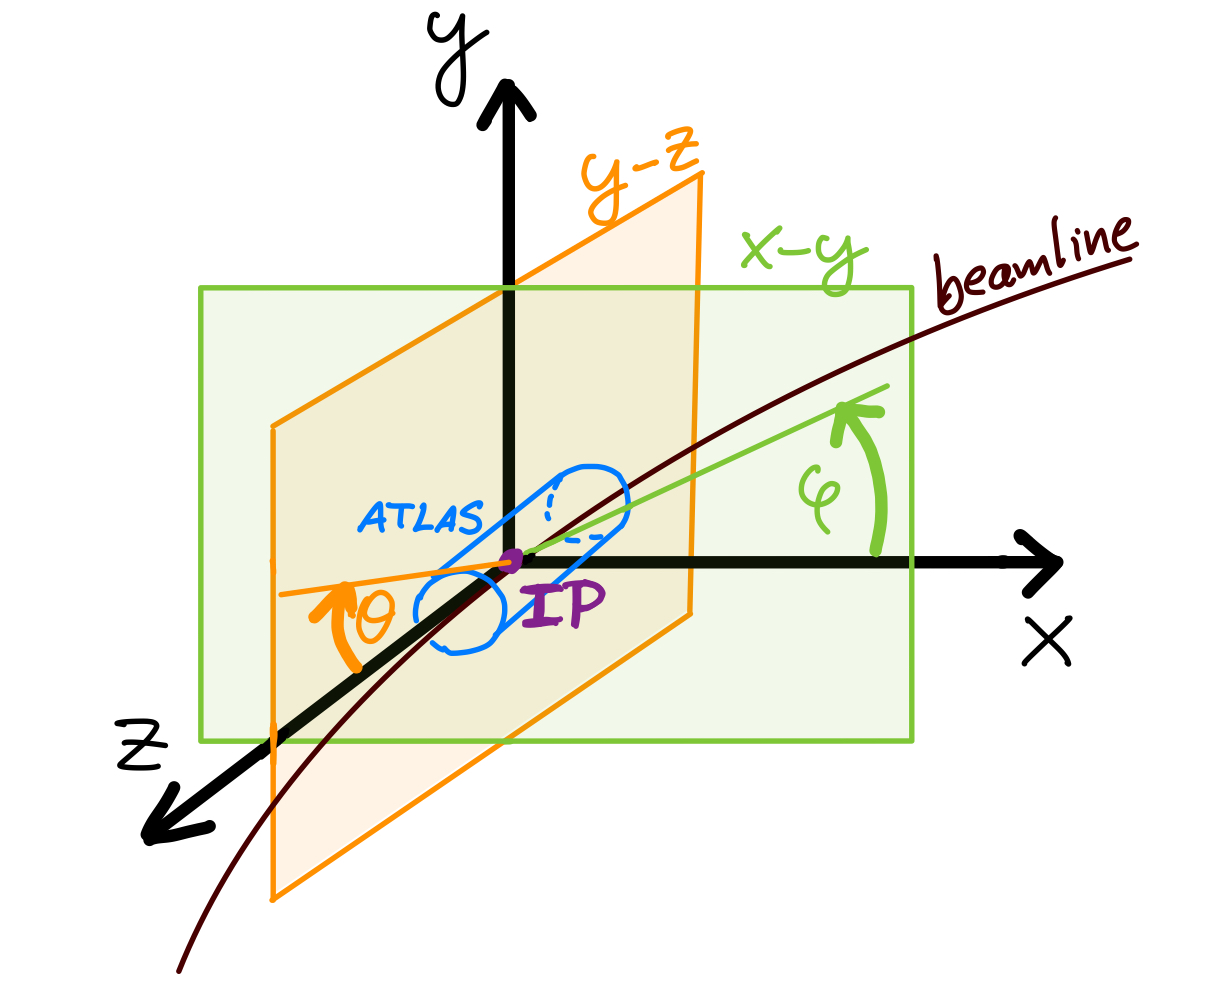
\includegraphics[width=0.7\linewidth]{src/img/ATLAS_coords.jpeg}
    \caption{The ATLAS coordinate system.}
    \label{fig:atlas_coord}
\end{figure}


\section{Large Hadron Collider}
\label{sec:lhc}
\LHC is the biggest particle accelerator in the world, operated by CERN, the European Organization for Nuclear Research.
It is built underground, up to 175m below the surface. \footnote{Due to the high prices of land in Geneva.}
To keep the particles in a circular motion, it uses superconducting NbTi magnets, reaching up to 8.33 T, submerged in a liquid He of temperature 1.9 K.
Particles are pre-accelerated in a sequence of linear and circular accelerators.
The system of all accelerators is shown in the \cref{fig:lhc}.
\begin{figure}[htb]
    \centering
    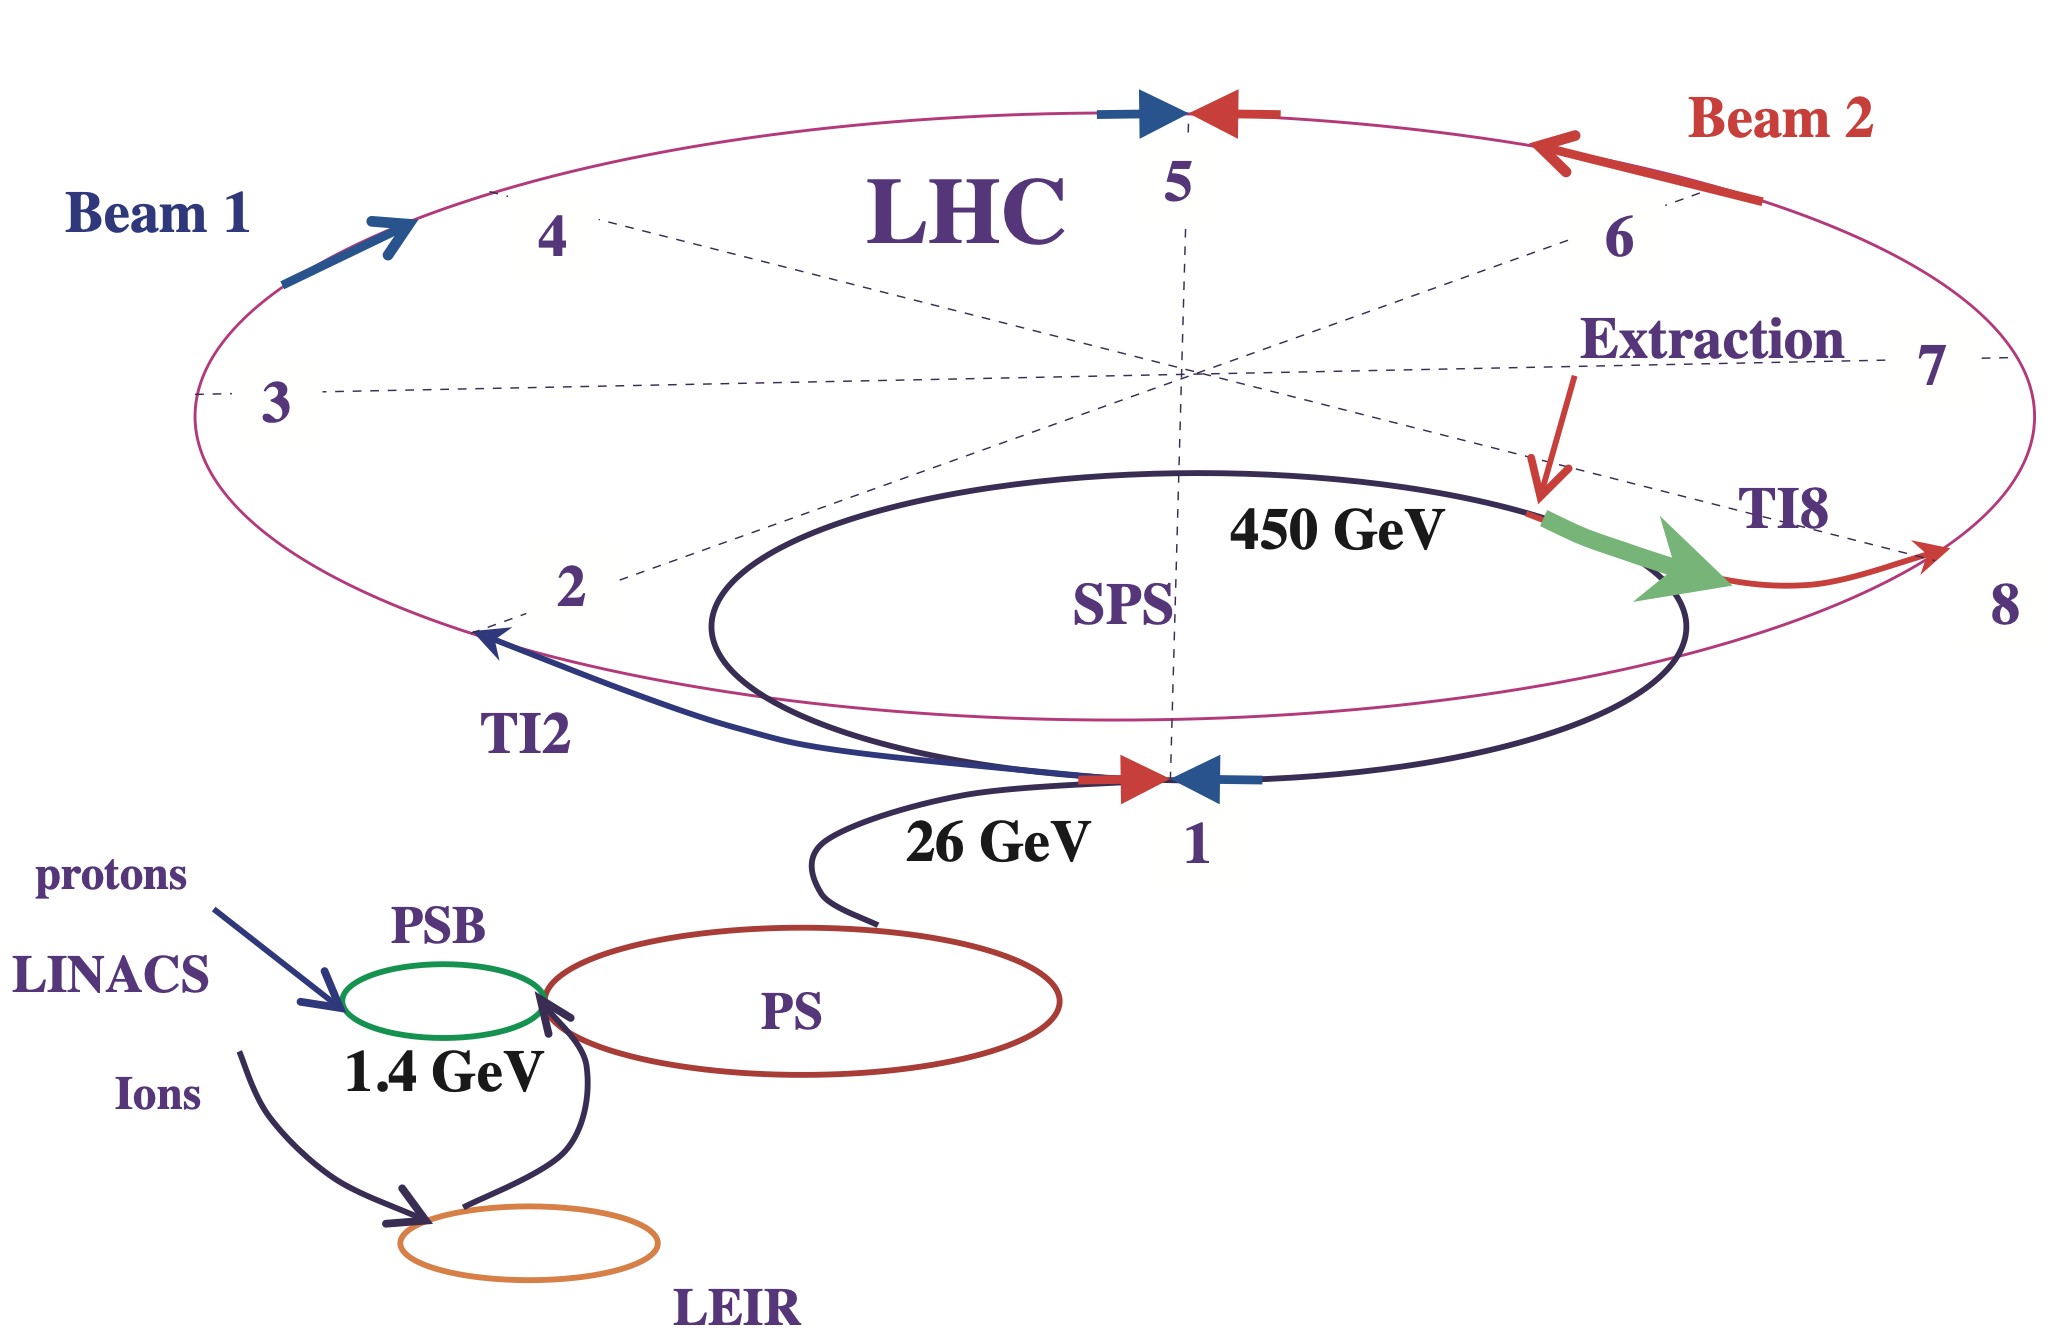
\includegraphics[width=0.9\linewidth]{src/img/LHC.png}
    \caption{The Large Hadron Collider, with its pre-accelerators.}
    \label{fig:lhc}
\end{figure}


At a given time, two beams of protons are circulating in opposite directions in the accelerator.
Beams are separated into \emph{bunches}, each containing approximately $1.3\cdot10^{11}$ protons.
At maximum, 2800 bunches are present in each beam, with a typical size of 200-300 $\mu$m and a spacing of 25 ns (about 7.5m).
The beams collide at four specific points where the detectors are.
Before the collision, the beams are focused to a size of 16 $\mu$m.

The most important physical variable of the accelerator is the \emph{luminosity} $L$, defined as 
\begin{equation}
    \label{eq:lumni}
    L = \frac{N_1 N_2 n_b f_{\text{rev}}}{A}, 
\end{equation}
where $N_1$, $N_2$ are the number of particles in each beam, $n_b$ is the number of bunches, $f_{\text{rev}}$ is the revolution frequency, and $A$ is the effective beam overlap cross section of the collision. 
If we assume the Gaussian distribution of the beams in the transverse plane, the overlap cross section is given by 
\begin{equation}
    A = 4 \pi \sigma_x \sigma_y,
\end{equation}
where $\sigma_x$ and $\sigma_y$ are the standard deviations of the Gaussian distribution.
\LHC has a luminosity of $L = 10^{34}$ cm$^{-2}$s$^{-1}$, which is the highest luminosity of any accelerator in the world, translating to billion collisions per second.

Another related variable is the \emph{integrated luminosity} $ \mathcal{L}$, expressing the amount the data collected in a given time period $T$
\begin{equation}
    \mathcal{L} = \int_{T} L dt,
\end{equation}
expressed in the units of inverse femtobarns (fb$^{-1}$).
For example, the ATLAS detector collected 140 fb$^{-1}$ of data.




\section{Inner Detector}
\label{sec:trackers}
\begin{figure}[htb]
    \centering
    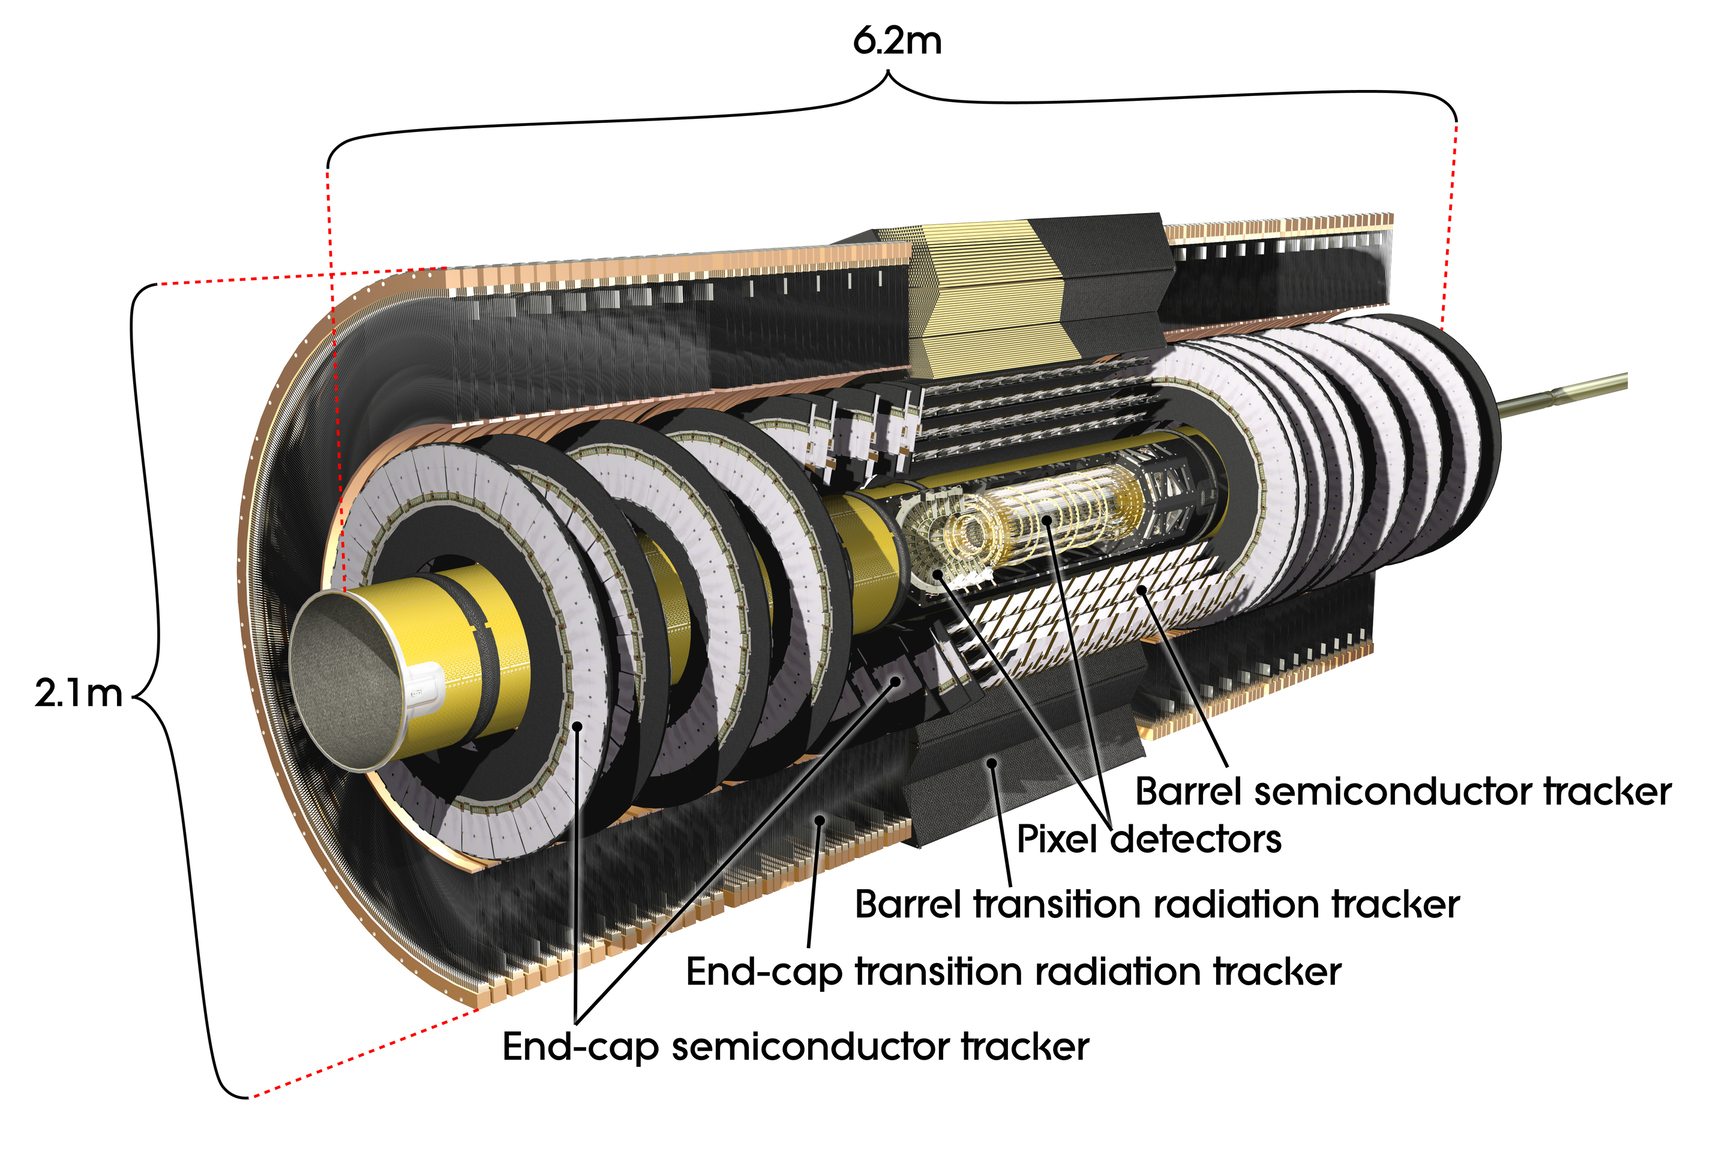
\includegraphics[width=1\linewidth]{src/img/track.jpg}
    \caption{Tracker system of the ATLAS detector.}
    \label{fig:tracker}
\end{figure}
The \emph{inner detector} consists of three parts: \emph{Pixel Detector}, \emph{Semiconductor Tracker}, and \emph{Transition Radiation Tracker}, \cref{fig:tracker}. 
They are the first detection points that are hit after the collision.
The primary purpose of the inner detector is to reconstruct the tracks of the charged particles.
As we can see in \cref{fig:det_inter}, only charged particles are visible by the inner tracking system.

Most interesting collisions are produced particles within $|\eta| < 2.5$, so the tracker is only in this region.
Even more, the inner detector is much denser and has a higher granularity in the central region, as seen in \cref{fig:tracker}.

\subsection{Pixel Detector}
The pixel detector, the first detection point, has the highest resolution and must withstand the highest radiation dose.
It consists of four layers of silicon pixels of size 50 x (250-400) $\mu$m$^2$.
With an accuracy of about 10 $\mu$m, it can locate a charged particle's origin and momentum.

The primary physical detection process is ionization.
As charged particles pass through the semiconducting silicon, they create electron-hole pairs, which are collected by the readout electronics.

\subsection{Semiconductor Tracker}
\SCT is similar to the pixel detector but with a different type of position measuring.
Instead of pixels, it uses  \emph{strips} to determine the particle's position.
It covers way more volume than the pixel detector, providing the most precise tracking system with a precision of up to 25 $\mu$m.
Determination of coordinates is done by precise alignment of the strips.

The physical process behind detection is the same as in the pixel detector.

\subsection{Transition Radiation Tracker}
\TRT is the last part of the inner detector, being the least precise.
Instead of silicon, it uses a gas mixture of Xe, CO$_2$, and O$_2$ to provide the ionizable material.
The gas is put into \emph{straws} with a diameter of 4 mm and a length of up to 144 cm.
Along the straw, in the middle, is a gold-plated tungsten wire acting as an anode, while the cathode is the tube wall.

When a charged particle passes through the gas, it produces ion pairs.
The anode is at ground potential attracting negative ions, while the cathode wall is at -1530V attracting positive ions.
The straws are interleaved with polypropylene fibers or foils to provide a material with different index of refraction.
Relativistic particles, with speeds above the speed of light in polypropylene (mainly electrons), generate transition radiation when moving from and into the polypropylene. 
Additional information about the particle is inferred from transition radiation, which is used to reconstruct the track and identify the particle. 



\section{Calorimeters}
\label{sec:calorimeters}
\begin{figure}[htb]
    \centering
    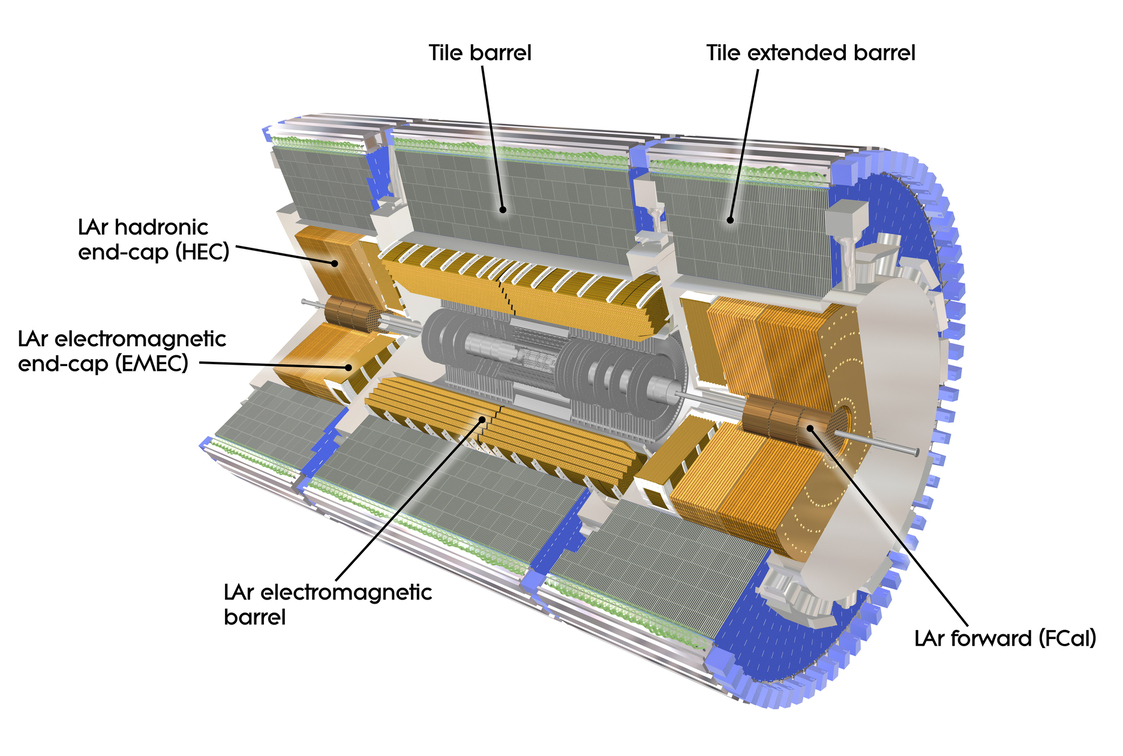
\includegraphics[width=1\linewidth]{src/img/calo.jpg}
    \caption{Calorimeter system of the ATLAS detector.}
    \label{fig:calorimeter}
\end{figure}

The primary purpose of calorimeters is to stop particles. 
More precisely, they are designed such that particles deposit most of the energy in them.
That is why they are much larger than the tracking system, as seen in \cref{fig:det_inter}. 
They are built up by alternating absorbing layers and energy-measuring layers. 

In \cref{fig:det_inter}, we can see two types of calorimeters:
\begin{itemize}
    \item \textbf{Electromagnetic calorimeter} designed to stop electrons, positrons, and photons.
    \item \textbf{Hadronic calorimeter} designed to stop hadron, i.e., composites of quarks and gluons.
\end{itemize}

The hadronic calorimeter is the most important for our study because it provides data for jet reconstruction.


\subsection{Electromagnetic Calorimeter}
Another name for the electromagnetic calorimeter is \LAr calorimeter because it uses liquid argon as a detecting material.
The \LAr is kept at -186$^\circ$C to maintain the liquid state.
As an absorber, the electromagnetic calorimeter uses lead.
Particles ionize the \LAr when passing the layers, creating a measurable current, which is then detected by accordion-shaped electrodes.

\subsection{Hadronic Calorimeter}
The hadronic calorimeter uses mainly \TCal, an envelope of the electromagnetic calorimeter, and \LAr at the endcaps and forwards part.
The \LAr part is similar to the electromagnetic calorimeter described above, but instead of lead, it uses copper and tungsten as an absorber.

The \TCal uses steel as an absorber and scintillating tiles as a detector.
As particles pass through the plastic scintillators, they excite the atoms inside, which emit light as they return to their ground state.
This visible light is then collected by fibers and converted with photomultiplier tubes into an electrical signal.
The intensity of the light is proportional to the energy deposited in the scintillator.




\section{Muon Spectrometer}
\label{sec:muon}
\begin{figure}[htb]
    \centering
    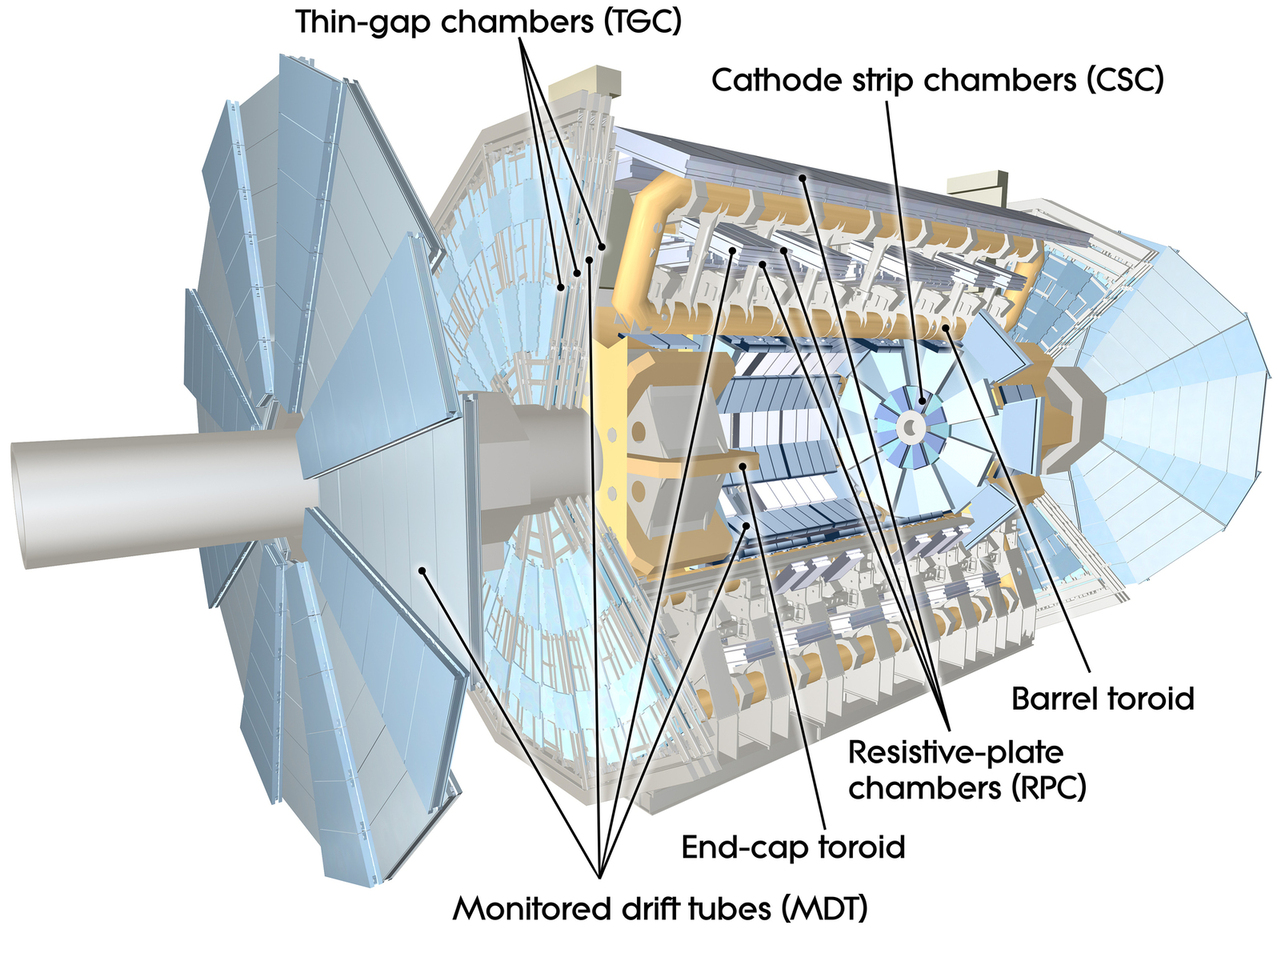
\includegraphics[width=0.8\linewidth]{src/img/muon.jpg}
    \caption{Muon spectrometer system of the ATLAS detector.}
    \label{fig:muon}
\end{figure}

The Muon Spectrometer is the furthest measuring system of the ATLAS detector, as seen in \cref{fig:muon}.
Muons have bigger mass than electrons and do not interact with the strong interaction as hadrons, so they are not stopped in the calorimeters (see \cref{fig:det_inter})

Since stopping the muons is not feasible, we measure their momentum and flight direction, utilizing the muon track's bending in a magnetic field, which we will explain in the next \cref{sec:magnet}.
Muon spectrometers surround the entire ATLAS detector to ensure that all muons are measured.
The tracker provides one measurement point, while the spectrometer offers the other to reconstruct the muon track with the precision of $10\%$ at 1 TeV.


\section{Magnet systems}
\label{sec:magnet}
\begin{figure}[htb]
    \centering
    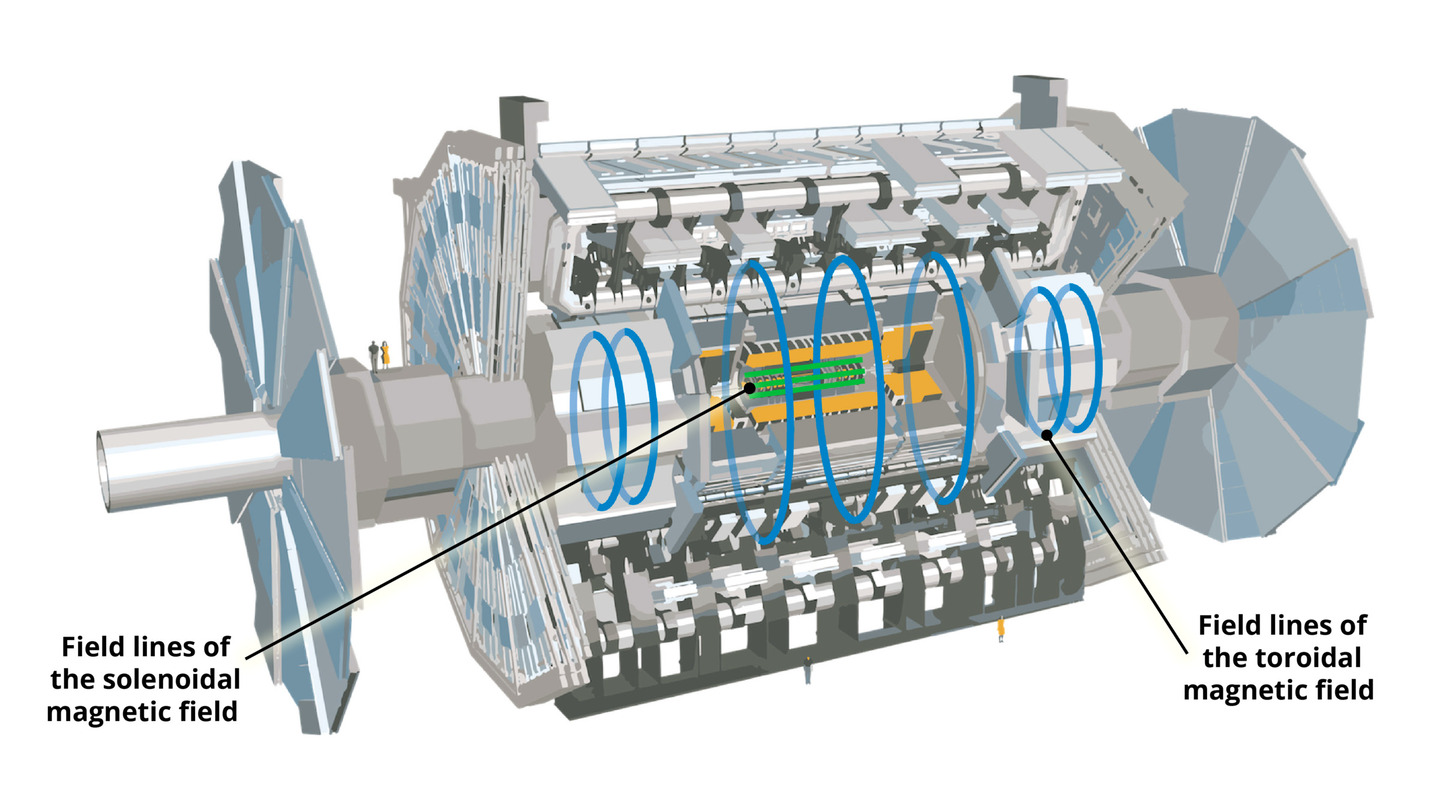
\includegraphics[width=1\linewidth]{src/img/magnet.jpg}
    \caption{Magnet system of the ATLAS detector.}
    \label{fig:magnet}
\end{figure}

In the whole ATLAS detector, there are two main systems of magnets, toroidal (blue field lines in \cref{fig:magnet}) and solenoidal (green field lines in \cref{fig:magnet}).
All magnets are superconducting, operated at -268$^\circ$C, to reach necessary field strengths.
The main purpose of magnets is to bend the trajectories of charged particles to measure their momentum $p$ according to \footnote{We assume that the magnetic field is constant and the particle's mass is zero.}
\begin{equation}
    \label{eq:magnet_momentum}
    \pT [\text{GeV}] = 0.3 \cdot q \cdot B [\text{T}] \cdot R [\text{m}],
\end{equation} 
where $q$ is the particle's charge (expressed in units of the elementary charge), $B$ is the magnetic field strength, and $R$ is the radius of the trajectory.

The inner NbTi magnets are solenoidal and provide coverage for the tracking system.
They produce a 2T magnetic field in the axial direction.
To give a perspective, if we assume an electron with a momentum of 10 GeV, the bending radius is 17 m.
This number is enormous compared to the radius of the solenoid magnet, which is just 1.2m. 
From this example, we can see how precise the tracking system is.

On the other hand, particles with momentum less than circa 360 MeV wind inside the solenoid magnet and do not reach the colorimeters.
One such example is low energetic pions, particularly important in our study because they are trapped inside the solenoid magnet, not reaching the calorimeters, and are not used in the jet reconstruction.

The toroidal magnets are composed of two parts: barrel and endcap.
The barrel magnets consist of eight 25.3m long, rectangular-shaped coils, the biggest toroidal magnets in the world.
They are supported by the endcap magnets, which cover particles going in the forward direction, as in \cref{fig:magnet}.
Together they provide a field of approximately 0.5-1T for bending the trajectories of muons, measured by the muon spectrometer. 


\section{Trigger}
\label{sec:trigger}
The high luminosity that \LHC provides results in a collision rate of 1.7 GHz, equivalent to 60 TB/s of data throughput.
This is a massive amount of data, impossible to store and process.
Most of the data contains no interesting physics, so it is filtered by the \emph{trigger system}.

The online trigger system consists of two levels, \emph{L1} and \emph{L2}. 
L1 uses only coarse data from calorimeters and muon spectrometers, searching for high $\pT$ particles.
It has to decide within 2.5$\mu$s, reducing the collision rate to 75 kHz.
Each kept event defines a coordinate region, called \RoI, by which L1 was activated. 

The L2 trigger uses the \RoI defined by L1 but with more precise data from the detector in that region.
Using a CPU farm of 40k CPU cores, L2 reduces the rate to 3.5 kHz, with a decision time of 200$\mu$s.

After L2, the data is stored for offline analysis.
\emph{Event filter} reduces the rate to 200 Hz with an event processing time of 4s.
The event filter is the last part of the trigger system. 
After it, the data is prepared for long-time storage and analysis.